\section{Loi de Student ($\st_n$)}

William Gosset, alors qu'il travaillait pour la brasserie Guinness \`a Dublin, avait l'interdiction de publier le r\'esultat de ses travaux. Apr\`es avoir suivi un cours de Statistiques donn\'e par Karl Pearson, il prit le pseudonyme de ''Student'' pour publier la distribution du m�me nom en 1908.

\subsection{Loi de Student \`a $n$ degr\'es de libert\'e}

La distribution de Student, aussi appel\'ee $t$-distribution,  est une famille de distribution en forme de cloche et sym\'etrique. Elle est similaire \`a la distribution normale, mais avec des valeurs plus grandes aux extr\'emit\'es ($x$ petit ou $x$ grand). Elle se caract\'erise par le nombre de degr\'es de libert\'e.

\begin{center}
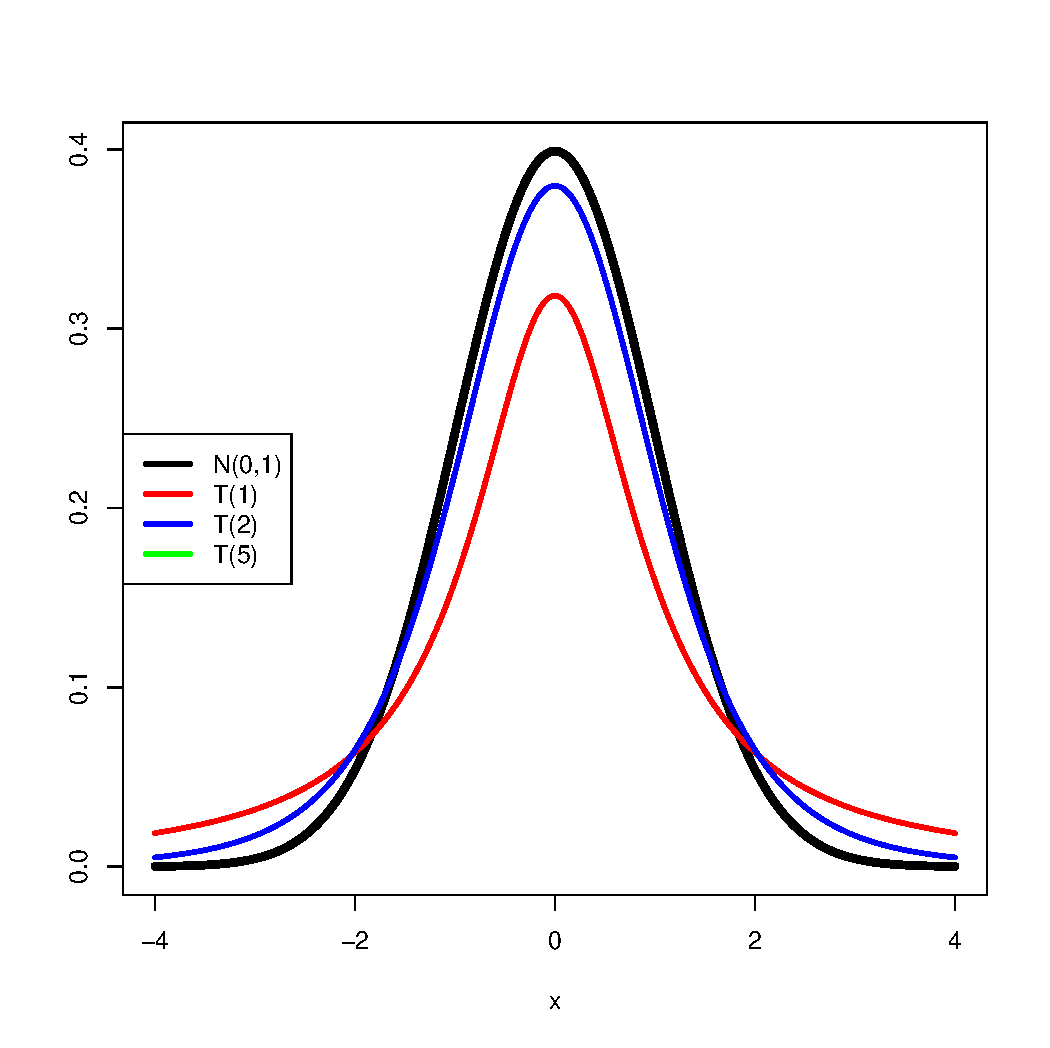
\includegraphics[scale=0.7]{normalevsStudent}
\end{center}

Lorsque le nombre de degr\'es de libert\'e $n$ tend vers l'infini, la loi de Student tend vers la loi normale $\norm(0,1)$.

%Soit $Z$ et $Q_n$, deux variables al\'eatoires ind\'ependantes telles que
%$$Z \sim N(0,1)\quad\quad Q_n\sim\chi^2_n$$
%
%Alors,
%$$T_n = \frac{Z}{\sqrt{\frac{Q_n}{n}}} \sim St_n$$
\newpage
\begin{pro}
$\st_n$: loi de Student \`a $n$ degr\'es de libert\'e
\begin{itemize}
	\item $\E(\st_n) = 0\, , \quad n>1$\\
	L'esp\'erance tend vers l'infini lorsque $n=1$. On dit alors qu'elle n'existe pas.
	\item $\var (\st_n) =  \frac{n}{n-2} \, , \quad n>2$\\
	La loi de Student a une variance infinie pour $n\leq 2$
	\item La loi de Student est sym\'etrique autour de 0.
\end{itemize}
\end{pro}

On utilisera le th\'eor\`eme suivant qui permet de faire de l'inf\'erence sur la moyenne d'une loi normale
de moyenne $\mu$ inconnue et de variance $\sigma^2$ inconnue.:
\begin{theo}
Soit un \'echantillon al\'eatoire de taille $n$, de moyenne $\bar{x}$ et de variance $s^2$, issu d'une loi normale $\norm(\mu,\sigma^2)$. Alors
$$\frac{\bar{x}- \mu}{\frac{s}{\sqrt{n}}}\sim \st_{n - 1}$$
\end{theo}

\subsection{Table de Student}
La table de la loi de Student se lit pour l'essentiel comme la table de la loi du $\chi^2$. Chaque ligne correspond \`a un nombre de degr\'es de libert\'e $n$ et chaque colonne \`a une erreur de premi\`ere esp\`ece $\alpha$. L'intersection d'une ligne et d'une colonne donne le seuil $t_{\alpha,n}$ tel que
$$P(\st_n\geq t_{\alpha,n})=\alpha$$
La relation entre $p$ et $\alpha$ est $p=1-\alpha$.

\begin{ex}
$$P(\st_{10}\leq t_{\alpha,10}) = 0.95  \quad \Longrightarrow t_{0.05,10} = 1.8125$$
\end{ex}

\'etant donn\'e que la loi de Student est sym\'etrique autour de 0, seules les erreurs de premi\`ere esp\`ece $\alpha$ inf\'erieures \`a 0.5 sont donn\'ees. Les $\alpha > 0.5$ peuvent �tre retrouv\'ees, comme pour la loi normale, par sym\'etrie et compl\'ementarit\'e.




